\hypertarget{genomic_projects_tutorials}{%
  \section{Genomic\_projects\_tutorials}\label{genomic_projects_tutorials}}

Under construction

This repository contains a collection of genomic projects that I am
working on. GitHub repository of bioinformatic projects recolving around
genomics using different tools like Plink through \texttt{plinkr} R
package, \texttt{rTASSEL} and TASSEL 5 (GUI), GEMMA for mixed models
analysis in R, SAMtools from the command line to analyze BAM files,
gBLUP coming soon.

The repository has been created for self-teaching purposes of biological
concept and bioinformatic tools, and make use of other repositories,
scripts and data sources, taken or modified as such.

\begin{enumerate}
  \def\labelenumi{\arabic{enumi}.}
  \tightlist
  \item
        SNP profiling of goat breeds.\emph{Data source}: \textbf{Colli et al.}
        (2018) https://doi.org/10.1186/s12711-018-0422-x
\end{enumerate}

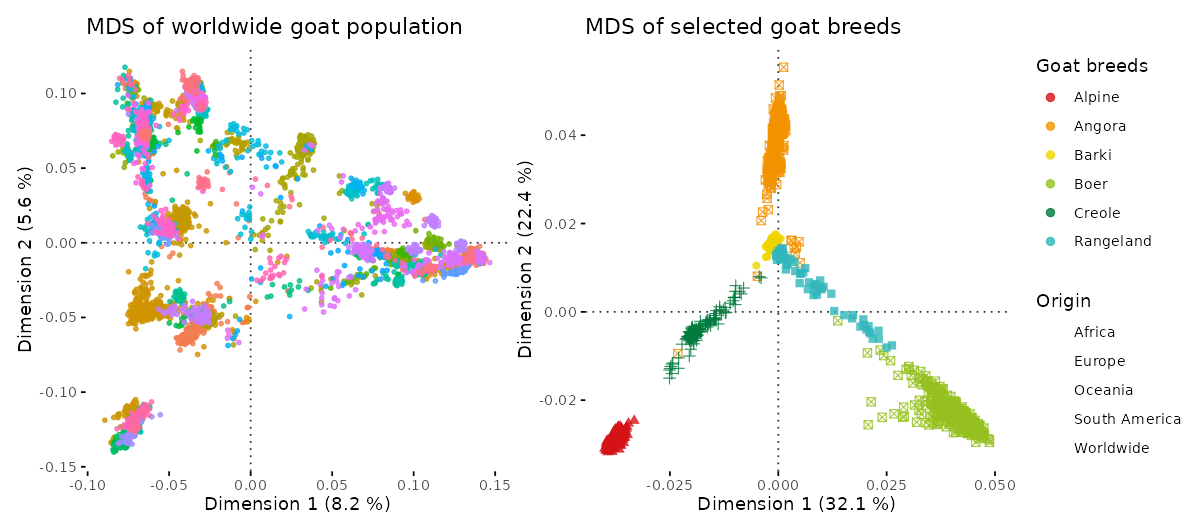
\includegraphics{Figures/goat_mds_2.png?raw=true}
\textbf{Multidimensional Scaling (MDS) Plot of a population of 4,653
  Individuals from 169 Goat Breeds genotyped with 49,953 SNPs.}

The MDS plot visualizes genetic relationships among 4,653 individuals
from 169 goat breeds. Genetic distances were computed using PLINK to
generate the kinship matrix, and MDS analysis was conducted with the
\texttt{cmdscale} function based on genotyping data from 49,953 SNPs.
Each point represents a goat, and spatial arrangement reflects genetic
dissimilarities. This exploratory analysis offers insights into genetic
diversity, population structure, and relatedness.

\begin{enumerate}
  \def\labelenumi{\arabic{enumi}.}
  \setcounter{enumi}{1}
  \item
        \begin{enumerate}
          \def\labelenumii{\alph{enumii}.}
          \tightlist
          \item
                Manhattan plot of a GWAS on dog population for deafness.Data
                source: \textbf{Hayward et al.} (2020)
                https://doi.org/10.1371/journal.pone.0232900
        \end{enumerate}
\end{enumerate}

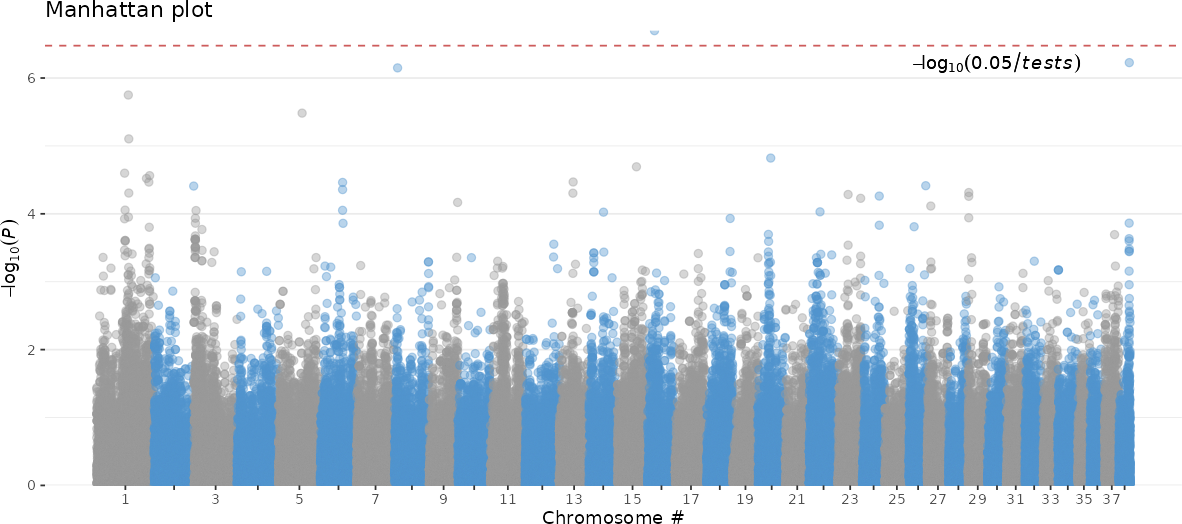
\includegraphics{Figures/manhattan_dogs.png?raw=true}
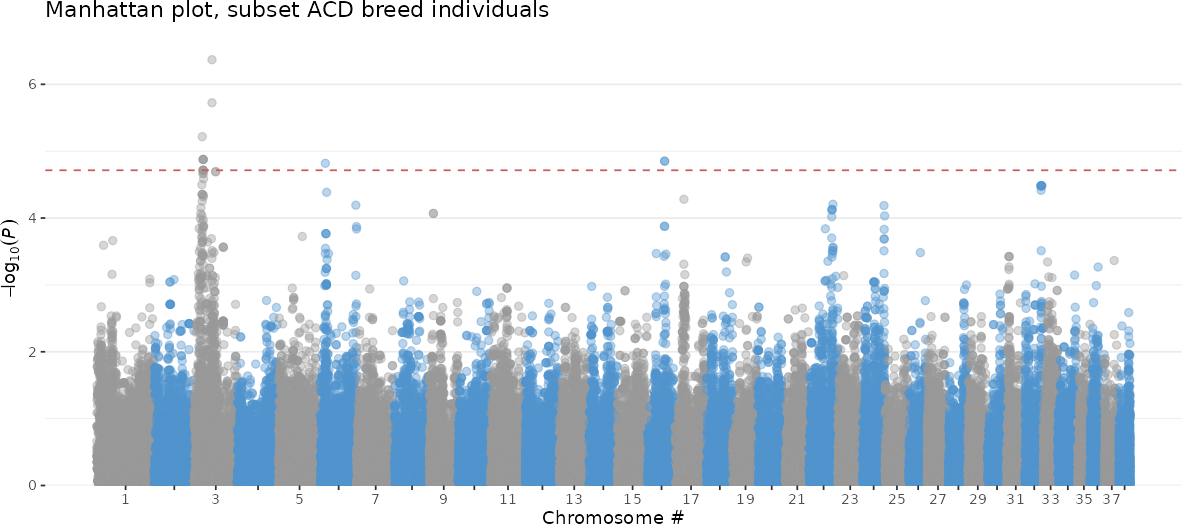
\includegraphics{Figures/manhattan_filter_acd.png?raw=true} Manhattan
plots showing the genome wide association (GWA) between dog deafness and
their genotype. The plot displays the genomic positions of single
nucleotide polymorphisms (SNPs) across the genome on the x-axis, with
the corresponding -log10 transformed \emph{P}-values indicating the
strength of association with the trait on the y-axis.

\begin{enumerate}
  \def\labelenumi{\arabic{enumi}.}
  \setcounter{enumi}{1}
  \item
        \begin{enumerate}
          \def\labelenumii{\alph{enumii}.}
          \setcounter{enumii}{1}
          \tightlist
          \item
                Plot of the top significant SNPs identified by the above GWAS.
        \end{enumerate}
\end{enumerate}

\begin{figure}
  \centering
  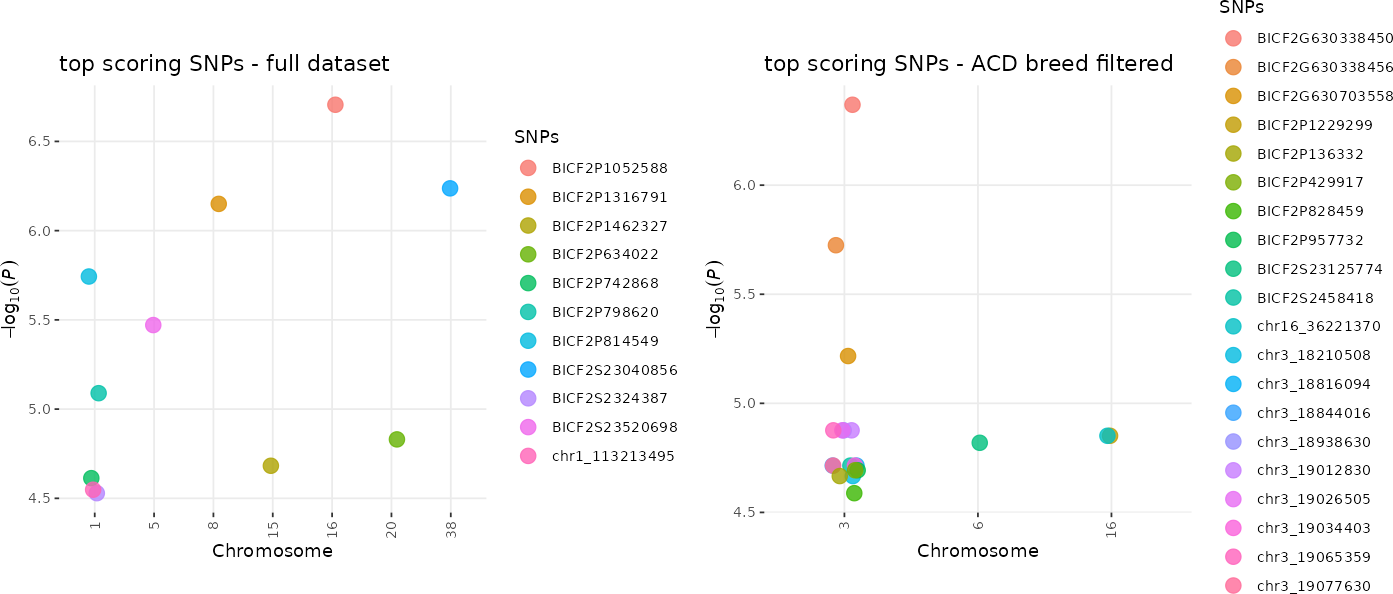
\includegraphics{Figures/top_SNPs_comb.png?raw=true}
  \caption{plot SNPs}
\end{figure}

\hypertarget{tools}{%
  \subsection{Tools}\label{tools}}

\begin{itemize}
  \item
        \textbf{PLINK 1.90} \url{https://www.cog-genomics.org/plink2/}
  \item
        \texttt{plinkr} R package repository documentation.
        \url{https://github.com/AJResearchGroup/plinkr}
  \item
        \textbf{TASSEL 5} \url{https://www.maizegenetics.net/tassel}.
        \textbf{Bradbury} et al., (2007) TASSEL: software for association
        mapping of complex traits in diverse samples, Bioinformatics, Volume
        23, Issue 19, Pages 2633--2635
        \url{https://doi.org/10.1093/bioinformatics/btm308}
  \item
        \texttt{rTASSEL} R package repository documentation. Vignettes:
        \url{https://rtassel.maizegenetics.net/index.html}, Repository:
        \url{https://github.com/maize-genetics/rTASSEL}. \textbf{Monier et
          al.}, (2022). rTASSEL: An R interface to TASSEL for analyzing genomic
        diversity. \emph{Journal of Open Source Software}, 7(76), 4530,
        \url{https://doi.org/10.21105/joss.04530}
  \item
        \texttt{GEMMA} Genome-wide Efficient Mixed Model Association
        \url{https://github.com/genetics-statistics/GEMMA}. \textbf{Xiang Zhou
          and Matthew Stephens} (2012). Genome-wide efficient mixed-model
        analysis for association studies. \emph{Nature Genetics} 44, 821--824.
\end{itemize}

\hypertarget{resources-data}{%
  \subsection{Resources \& Data}\label{resources-data}}

\begin{itemize}
  \item
        \textbf{Marees et al.} (2018) A tutorial on conducting genome-wide
        association studies: Quality control and statistical analysis.
        \emph{Int J Methods Psychiatr Res}. 27:e1608.
        \url{https://doi.org/10.1002/mpr.1608}
  \item
        \textbf{Marees et al.} (2018) tutorial
        \url{https://github.com/MareesAT/GWA_tutorial}
  \item
        \textbf{Gábor Mészáros} (2021) Genomic Boot Camp Book
        \url{https://genomicsbootcamp.github.io/book/}
  \item
        \textbf{Gábor Mészáros} video tutorials
        \url{https://www.youtube.com/c/GenomicsBootCamp}
  \item
        \textbf{Colli et al.} (2018) Genome-wide SNP profiling of worldwide
        goat populations reveals strong partitioning of diversity and
        highlights post-domestication migration routes. \emph{Genet Sel Evol}
        50, 58. \url{https://doi.org/10.1186/s12711-018-0422-x}
  \item
        DATA: \textbf{Colli et al.} (2020). Signatures of selection and
        environmental adaptation across the goat genome post-domestication
        {}Dataset{}. \emph{Dryad}.
        \url{https://doi.org/10.5061/dryad.v8g21pt}
  \item
        \textbf{Decker et al.} (2014) Worldwide Patterns of Ancestry,
        Divergence, and Admixture in Domesticated Cattle. \emph{PLOS Genetics}
        10(3):
        e1004254.\href{https://journals.plos.org/plosgenetics/article?id=10.1371/journal.pgen.1004254}{https://doi.org/10.1371/journal.pgen.1004254},
  \item
        DATA: \textbf{Decker et al.} (2015) Worldwide patterns of ancestry,
        divergence, and admixture in domesticated cattle {}Dataset{}. Dryad.
        \url{https://doi.org/10.5061/dryad.th092}
\end{itemize}

\hypertarget{setup-of-the-working-environment}{%
  \subsection{Setup of the working
    environment}\label{setup-of-the-working-environment}}

Install R: \href{https://cran.r-project.org/}{The Comprehensive R
  Archive Network (CRAN)}

IDE:\href{https://code.visualstudio.com/}{VSCode}/\href{https://posit.co/download/}{RStudio}*

Install Python:
\href{https://docs.anaconda.com/free/miniconda/index.html}{Miniconda 3}*

OS: Linux*/WSL

*Suggested

\hypertarget{get-plink-working-in-linux}{%
  \subsubsection{Get PLINK working in
    Linux}\label{get-plink-working-in-linux}}

\begin{enumerate}
  \def\labelenumi{\arabic{enumi}.}
  \item
        Download
        \href{https://s3.amazonaws.com/plink1-assets/plink_linux_x86_64_20231211.zip}{PLINK
          1.90 Linux 64-bit}
  \item
        Install PLINK
        \texttt{cd\ Downloads/\ \ \ \ \ sudo\ unzip\ plink\_linux\_x86\_64\_20200616.zip\ -d\ plink\_install}
  \item
        PLINK in \texttt{usr/local/bin}

        \begin{verbatim}
cd plink_install
sudo cp plink /usr/local/bin
sudo chmod 755 /usr/local/bin/plink
\end{verbatim}
  \item
        Add PLINK to PATH

        with bash/zsh/\ldots{}

        \begin{verbatim}
sudo nano ~/.bashrc
\end{verbatim}

        adn include the line:

        \begin{verbatim}
export PATH=/usr/local/bin:$PATH
\end{verbatim}

        Save and exit. Refresh the terminal and you should be able to call
        \texttt{plink} from the terminal at any user position in the system.

        \begin{verbatim}
source ~/.bashrc
plink --help
\end{verbatim}
\end{enumerate}

\hypertarget{get-tassel-gui-on-linux}{%
  \subsubsection{Get TASSEL (GUI) on
    Linux}\label{get-tassel-gui-on-linux}}

\begin{enumerate}
  \def\labelenumi{\arabic{enumi}.}
  \item
        Go on the website \url{https://www.maizegenetics.net/tassel} and
        download the last UNIX verison.
  \item
        Download the TASSEL\_\{xxx\}\_unix.sh and make it executable

        \begin{verbatim}
chmod +x ~/Downloads/TASSEL_{xxx}_unix.sh
\end{verbatim}
  \item
        Run the TASSEL installer

        \begin{verbatim}
~/Downloads/TASSEL_{xxx}_unix.sh
\end{verbatim}
\end{enumerate}

\hypertarget{get-rtassel-working-in-linux}{%
  \subsubsection{\texorpdfstring{Get \texttt{rTASSEL} working in
      Linux}{Get rTASSEL working in Linux}}\label{get-rtassel-working-in-linux}}

\begin{enumerate}
  \def\labelenumi{\arabic{enumi}.}
  \item
        \texttt{rJava} installation

        \begin{verbatim}
sudo apt install default-jdk
sudo R CMD javareconf
R install.packages("rJava")
\end{verbatim}
  \item
        Installation in R

        \begin{verbatim}
if (!require("devtools")) install.packages("devtools")
devtools::install_github(
 repo = "maize-genetics/rTASSEL",
 ref = "master",
 build_vignettes = TRUE,
 dependencies = TRUE
)
\end{verbatim}
  \item
        Run \texttt{rTASSEL}

        \begin{itemize}
          \tightlist
          \item
                Allocate job's memory1 and start the logger (here at the root of the
                project):
        \end{itemize}

        1``-Xmx50g'' and ``-Xms50g'', ``\emph{50g}'' represents 50 Gigabytes
        of memory.

        \emph{!! Choose an appropriate value that fits your machine !!}

        \begin{verbatim}
options(java.parameters = c("-Xmx50g", "-Xms50g"))
rTASSEL::startLogger(fullPath = NULL, fileName = NULL)
\end{verbatim}

        \begin{itemize}
          \tightlist
          \item
                Run \& infos
        \end{itemize}

        \begin{verbatim}
library(rTASSEL)
??rTASSEL
\end{verbatim}

        Useful resource for \texttt{rTASSEL} are the vignettes and tutorials
        at \url{https://rtassel.maizegenetics.net/index.html}
\end{enumerate}

\hypertarget{get-gemma}{%
  \subsubsection{\texorpdfstring{Get
      \texttt{GEMMA}}{Get GEMMA}}\label{get-gemma}}

GEMMA can be installed from source at the GitHub repo, but is also
available through Bioconda \url{http://www.ddocent.com/bioconda/}. To
install is suggested to have miniconda installed and working, and then
added the channel for Bioconda, you should already have defaults and
conda-forge.

\begin{verbatim}
conda config --add channels defaults
conda config --add channels conda-forge
conda config --add channels biocond
conda install gemma
\end{verbatim}

And use GEMMA with

\begin{verbatim}
gemma -h
\end{verbatim}

\begin{center}\rule{0.5\linewidth}{0.5pt}\end{center}
